\chapter{Interest Rate Volatility and Derivatives}\label{chap::LMM}

Before introduction of the market models, short rate models are widely used by practitioners for interest rate derivatives pricing. Examples of short-rate models are \cite{vo97} model, \cite{cir85} model and \cite{jh90} model. These models establish the instantaneous spot interest rate dynamics, using single or multi-dimensional diffusion process(es). However, the interest rate dynamics from short rate models is not compatible with Black's formula for either swap or swaption. In other words, simplified and inexact assumptions are made on interest rate distribution in short rate models, in order to extrapolate the term structure of rates. This knowledge of term structure is vital to interest rate derivatives pricing. The lack of calibration to the whole forward curve is a trade-off with mimicking the Black-Scholes model for stock option in interest rate option, but brings in market inconsistency.

The LIBOR market model (LMM), instead, is based on the discretization of the yield curve into discrete forward rates. And each of these forward rate represents to the market quote of corresponds Forward Rate Agreement (FRA). More importantly, the LIBOR market model prices caps with Black's cap formula (lognormal forward-LIBOR model, LFM) and prices swaption with Black's swaption formula (lognormal forward-swap model, LSM). That is, the interest rate dynamics from the LMM are consistent with caps and swaptions, which are two most standard and basic interest-rate option on the market.

\section{LMM Framework}
\subsection{Forward Rate}
In standard LMM, we assume that the stochastic differential equation of each $n$ spanning forward rates $f_i$ formulates as
\begin{equation} \label{eqn::forward_rate}
\frac{d f_i}{f_i} = \mu_i (\mathbf{f}, t)dt + \sigma_t(t) d\tilde{W_i}
\end{equation}
where $\mathbb{E}[ d\tilde{W_i}  d\tilde{W_j}] = \rho_{ij} dt$. The lognormal-type model setup ensures positive forward rates. And $i,j=1,2,\ldots,M$. The derivative of Black's formula for caplets is detailed in Appendix

\subsection{Numeraire and Measure}
Consider the forward (adjusted) probability measure $Q^i$ associated with numeraire $P(\cdot,T_i)$ for maturity $T_i$, where the price of the bond maturity coincides with the forward rate maturity. With simple compounding, it follows
$$
d f_i P(t,T_i) = [P(t,T_{i-1}) - P(t,T_{i-1})] / \tau_i
$$
Note that $f_i P(t,T_i)$ is a tradable asset's price, where the price divides by the numeraire $P(\cdot,T_i)$ is $f_i(t)$ itself. Therefore, $f_i(t)$ follows a martingale under forward measure. Corresponding driftless dynamics for $f_i(t)$ under this measure with respect to Equation~\ref{eqn::forward_rate} is
$$
\frac{d f_i(t)}{f_i(t)} = \sigma_i(t) dW_i(t)
$$
When $\sigma$ is bounded and using Ito's formula, the unique strong solution of the forward rate dynamic is
$$
\log f_i (T) = \log f_i(0) - \int_0^T \frac{\sigma_i(t)^2}{2} dt + \int_0^T \sigma_i(t) dW_i(t)
$$
The instantaneous volatility term $\sigma_i(t)$ assumes to be piecewise-constant
$$
\sigma_i(t) = \sigma_{i,\beta(t)}(t)
$$
where in general $\beta(t)=m$ if $T_{m-2}<t \leq T_{m-1}, m\geq 1$.

Under this lognormal assumption, it yields that the dynamics of $f_k$ under forward measure $Q^i$ in three cases $i<k, i=k$ and $i>k$ are
\begin{eqnarray*}
i<k,& t\leq T_i: df_k(t) = \sigma_k(t)f_k(t)\sum_{j=i+1}^{k}\frac{\rho_{k,j}\tau_j\sigma_j(t)f_j(t)}{1+\tau_j f_j(t)}dt + \sigma_k(t) f_k(t) dW_k(t) \\
i=k,& t\leq T_{k-1}: df_k(t) = \sigma_k(t) f_k(t) dW_k(t) \\
i>k,& t\leq T_{k-1}: df_k(t) = -\sigma_k(t)f_k(t)\sum_{j=i+1}^{k}\frac{\rho_{k,j}\tau_j\sigma_j(t)f_j(t)}{1+\tau_j f_j(t)}dt + \sigma_k(t) f_k(t) dW_k(t)
\end{eqnarray*}
where $W=W^i$ is a Brownian motion under $Q^i$. 

\subsection{Risk Neutral Dynamics in LMM}
According to~\cite{bm06}, the risk-neutral dynamics of forward LIBOR rates in the LMM is 
$$
d f_i(t) = \tilde{\mu}_i(t) f_i(t)dt + \sigma_i(t)f_i(t) d \tilde{W}_i(t)
$$
where
\begin{eqnarray*}
\tilde{\mu}_i(t) &=& \sum_{j=\beta(t)}^{i} \frac{\rho_{i,j}\tau_j\sigma_i(t)\sigma_j(t)f_j(t)}{1+\tau_j f_j(t)} + \tilde{\sigma}_i(t)\rho\int_t^{T_{\beta(t)-1}}\tilde{\sigma}_f(t,u)'du \\
                 &=& \sum_{j=\beta(t)}^{i} \frac{\rho_{i,j}\tau_j\sigma_i(t)\sigma_j(t)f_j(t)}{1+\tau_j f_j(t)} + \sum_{j=\beta(t)}^{i} \rho_{i,j}\sigma_i(t)\rho\int_t^{T_{\beta(t)-1}}\tilde{\sigma}_f(t,u)'du
\end{eqnarray*}
where $\tilde{\sigma}$ is the horizontal $M$-vector volatility coefficient for the forward rate $f_i(t)$. 


\section{Calibration of LMM to Caps Prices}


Figure~\ref{fig::curves} plots the zero and forward curves as of market date 2016-06-30. 

\begin{center}
  \begin{figure}
      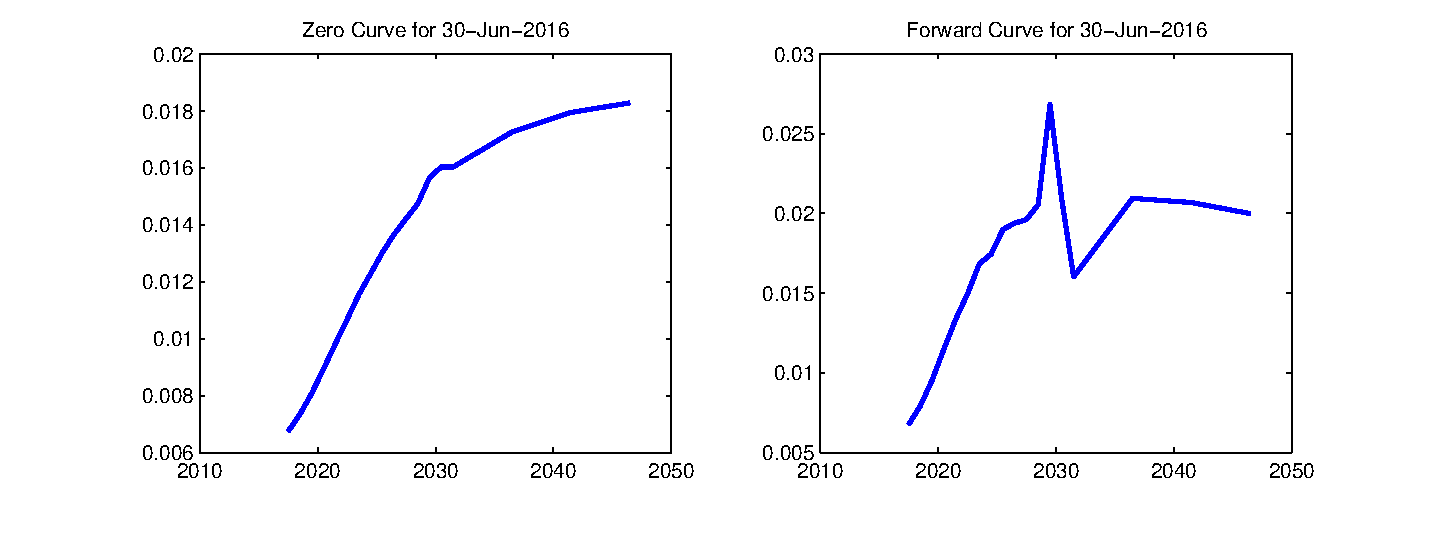
\includegraphics[scale=0.6]{zero_forward_curves.eps}
      \caption{The zero curve (left) and forward curves (right) as of 2016-06-30.}\label{fig::curves}
  \end{figure}
\end{center}


Figure~\ref{fig::vol_term} plots the term structure of the volatility from the calibrated LMM.

\begin{center}
  \begin{figure}
      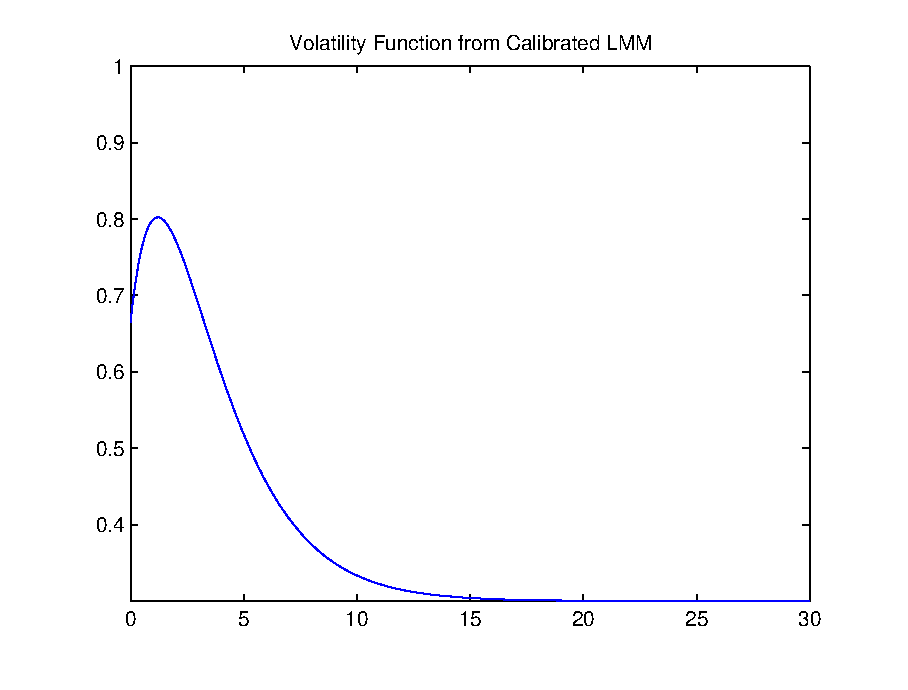
\includegraphics[scale=0.6]{vol_func.eps}
      \caption{The term structure of volatility from calibrated LMM.}\label{fig::vol_term}
  \end{figure}
\end{center}


Figure~\ref{fig::sim_zero_forward} plots the simulated zero curves and forward curves in one scenario (out of 1000) from the calibrated LMM.

\begin{center}
  \begin{figure}
      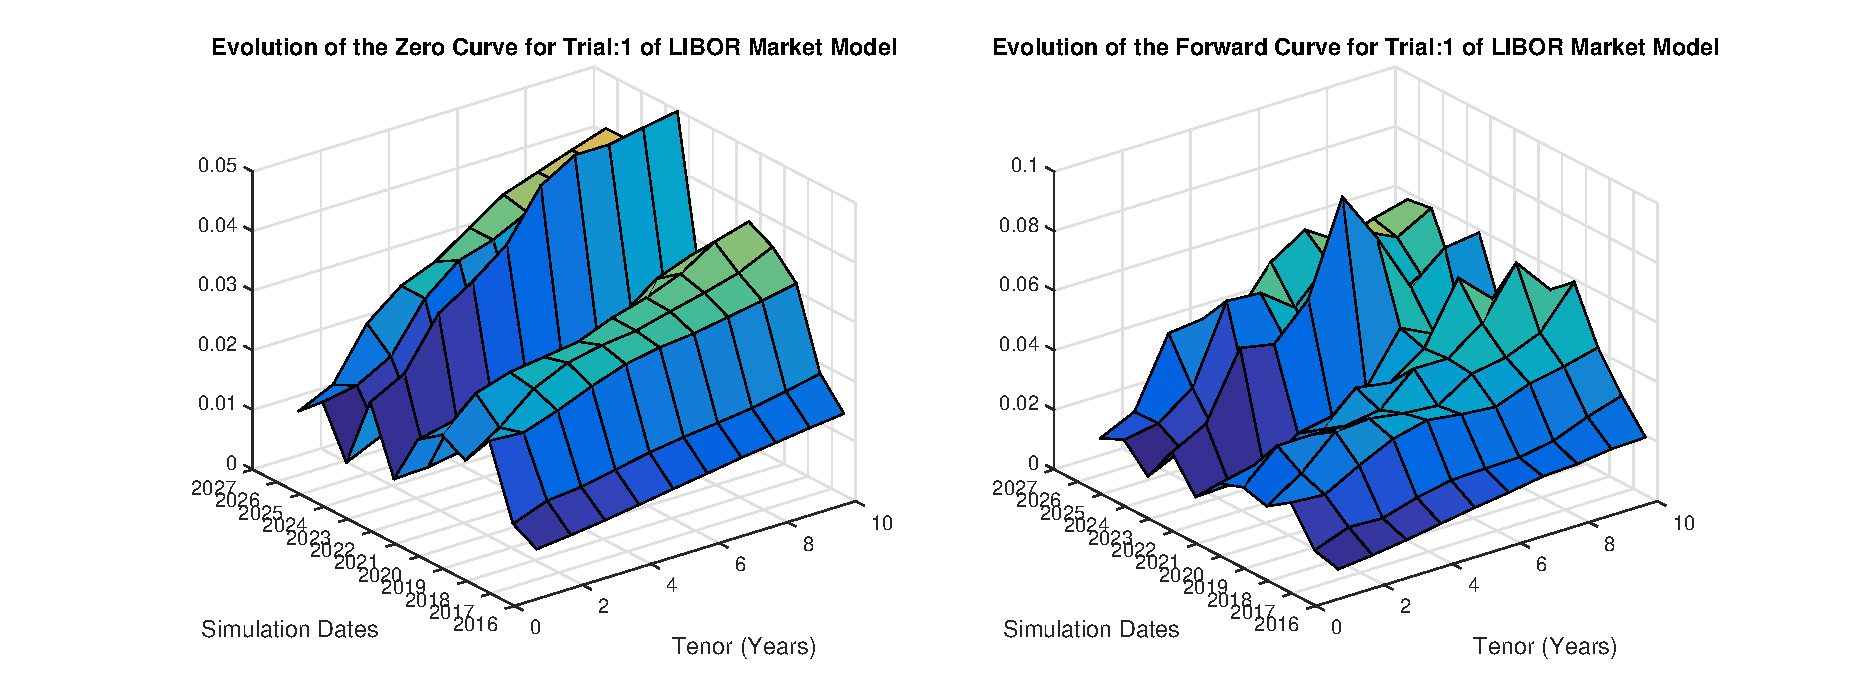
\includegraphics[scale=0.6]{sim_zero_forward.eps}
      \caption{Simulated zero curves and forward curves in one scenario from calibrated LMM.}\label{fig::sim_zero_forward}
  \end{figure}
\end{center}


\section{Test: Reprice Cap and Swaption} 